\documentclass[thesis.tex]{subfiles}
\begin{document}

\chapter{Introduction}
\label{chap:introduction}

\begin{figure}[h]
\centering
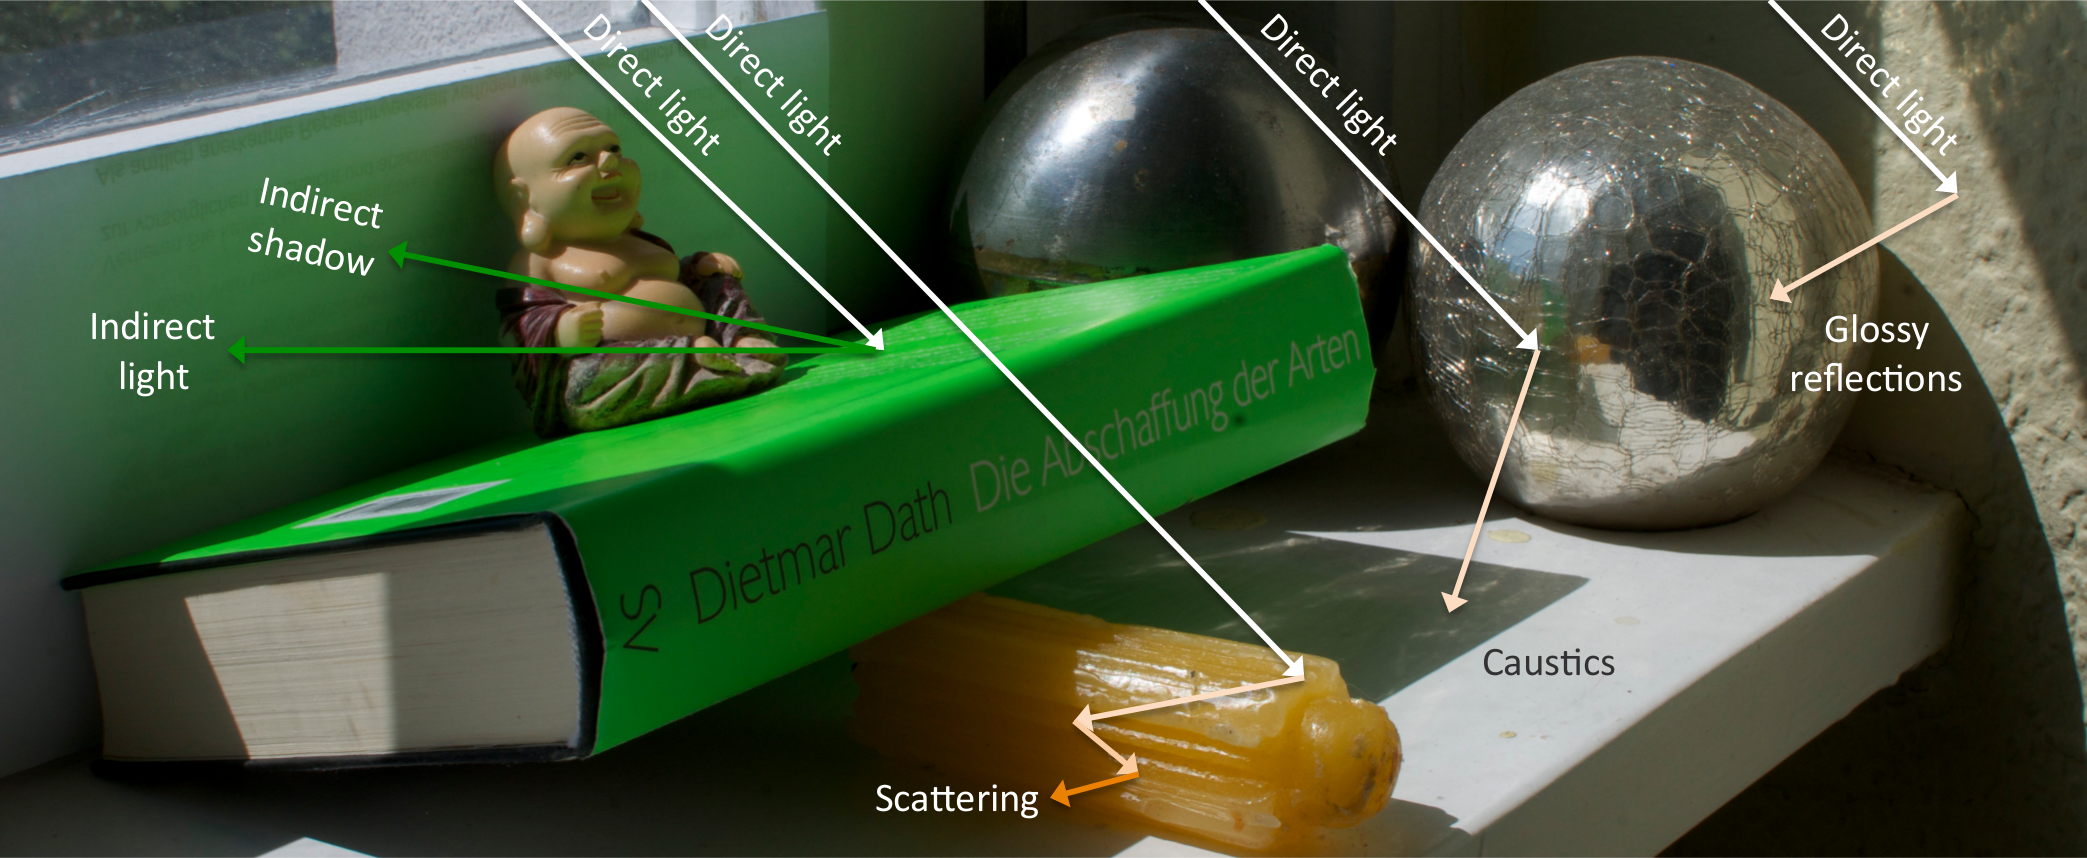
\includegraphics[width=\textwidth]{giphenomenons}
\caption{\cite{bib:RealtimeGIOverview} Photography of a scene with various global illumination effects: Diffuse and specular bounces, caustics and scattering.}
\label{fig:giphenomenons}
\end{figure}

\section{Introduction}
Everything that human eyes can perceive is the result of light reaching the retina after interacting with matter.
The way how light interacts with our environment is very complex and depends always on a global context.
There is a variety of natural phenomenons like indirect light, (indirect) shadowing, (glossy) reflections, and scattering which are impossible to simulate by local lighting models.
The photography in \autoref{fig:giphenomenons} demonstrates a few of them.
Compared to the simulation of local light effects which only take an isolated surface point into consideration, the simulation of global illumination effects as they occur in nature is extremely challenging both in terms of computational and algorithmic complexity.
\\
Images which lack these global effects look synthetic and are often missing important cues which are needed to understand the interrelations of the depicted objects.
Wherever 3D-scenes need to be displayed in a either believable or aesthetic manner, the simulation of global illumination becomes important.
Some of these applications are namely movies, architectural visualizations, video games and professional training simulations.
While the concrete demands of these applications vary greatly, the underlying principles are the same as they are governed by the physical laws of light which are familiar to our visual system.
\\
Generally, these applications can be divided in two categories: Interactive and non-interactive.
Where a non-interactive application like a movie or single images can afford computation times of several days, interactive applications need to compute at least parts of the simulation just-in-time to provide the user with the expected feedback on his actions.
A simulation is usually called interactive if images are rendered in less than 50ms (20 frames per second).
However, frame rates need to be much higher to be comfortable for the user.
Fast paced games usually profit from much better rendering times of more than 16ms (about 60 frames per second) \cite{bib:shooterfps} and the vendors of the upcoming virtual reality displays recommend even shorter rendering times of about 11-8ms (90-120 frames per second) to reduce motion sickness \cite{bib:oculushighfps}.
Naturally, real-time rendering that is performed on personal computers usually makes use of a different set of approaches and algorithms as offline rendering which runs often on large computer clusters.
In this work we want to introduce a new global illumination approach that is aimed for real-time rendering and does not need any pre-computation.
% resolutions rising?

\section{Motivation} \todo{Merge Intro/Motiv? "Pronounce differences" between sections?}
\begin{figure}[h]
\centering
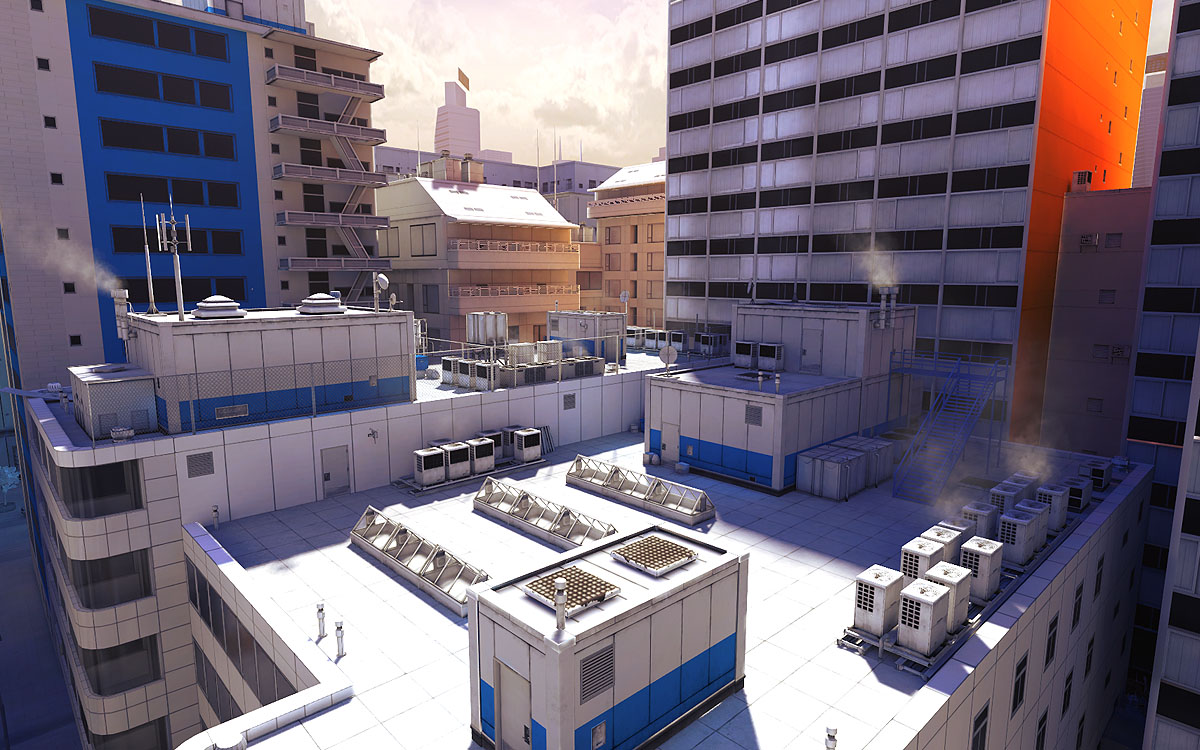
\includegraphics[width=\textwidth]{mirrorsedgescreenshot}
\caption{Screenshot from the 2008 video game \emph{Mirrors Edge}, featuring precomputed indirect lighting.}
\label{fig:gameprecomputedgi}
\end{figure}
To be able to display the aforementioned light effects in real-time, interactive application make often use of various pre-computation steps under the assumption that specific parts of the scene do not change.
In the extreme case this means that both scene and lighting conditions are assumed to be completely static which allows to compute a large variety of effects up-front.
This has been common practice in many games for over a decade now, as seen e.g. in Mirrors Edge in \autoref{fig:gameprecomputedgi} where only the characters and very few dynamic objects are lit at runtime.
\\
Obviously such techniques imply many restrictions on the design of virtual worlds and may not be applicable at all.
However, there are also solutions which less restrictions, for example to allow dynamic lights in a static scene or apply precomputed lighting on dynamic objects (more on other techniques in \autoref{chap:prevwork}).
Of course there are various trade-offs between different approaches and so far there is no technique that is even close to simulate all global illumination effects in real-time in a reasonable quality (which can be considered to be an open problem for offline rendering as well).
\\
A fully dynamic lighting approach not only frees a simulation of many technical restrictions, but also lowers the scene authoring iteration times as it is no longer necessary to wait for pre-computation processes to display the final result.
Currently there are relatively few approaches that allow global illumination effects within completely dynamic scenes and lighting conditions.
Of those, many come with a prominent artifacts like temporal incoherency (flickering).
This is why many applications for which pre-computations are not applicable fall back to comparatively simple direct lighting and drop almost all important effects of global illumination.

\section{Goals} \label{bib:goals}
The primary goal of this work is to explore the field of completely dynamic global illumination further and come up with a new solution which satisfies the conditions presented in this section.

We limit ourselves to what we think are the most important global illumination effects: Indirect diffuse lighting, indirect shadows and glossy reflections.
Light can bounce many times in a scene before it reaches the viewer.
In this thesis however, only the most important first indirect bounce will be handled.
% ability to parameterize BRDFs locally?
\\
As already mentioned, we strongly focus on avoiding precomputation entirely and demand that all computations can be performed every frame.
It should be possible to manipulate the scene's geometry and surface materials as well as lights and the camera freely at runtime.
\\
The solution should run entirely on the graphics hardware to free the CPU for different work and avoid expensive transfers.

Our most important quality criterion is temporal coherency.
Many dynamic global illumination approaches suffer from flickering when moving either light, objects or the camera.
We believe that such artifacts are far more intolerable than physical inaccuracies of a lighting solution.
Therefore, this work aims to avoid such artifacts as good as possible.
\\
%The criterion which is most obvious and easiest to measure is of course the time a single frame needs to render.
The time that a single frame takes to render should be adequate to the computed detail at all times.
This also means that we want to be able to trade quality for performance if necessary.
We aim for real-time rendering performance on mid-range desktop hardware.
\\
The work tries to accomplish appealing and credible lighting, physical correctness is secondary.
Though, it should be based on physical laws to be able to make statements about its theoretical correctness.
%We want to be able to run the algorithm on weaker machines or in situations where a real-time solution can not be presented at the highest quality.
\\
In contrast to precomputation-based techniques and also some modern dynamic approaches we want to try to keep the memory consumption low.
\\
Finally, the approach should be as invariant as possible to the chosen scene and its scale. %in terms of performance and memory requirements.
That means that the technique should adapt well to various small and large scenes and still deliver convincing results.

\todo{[Jo] Consider additional goals: Invariance to resolution}

%As the problem of real-time global illumination is known to be challenging


%\begin{itemize}
%\item Realtime global illumination, first bounce
%\subitem Dynamic camera, scene and lights!
%\item No significant precomputation
%\subitem This is important, as it excludes LightSkin!
%\item Support both diffuse and glossy reflections
%\subitem Simple BRDFs are okay, but we want to parameterize them 
%\item Temporal consistency
%\item Preferable scalable with large scenes
%\item Adequate lighting quality
%\item Colored indirect shadows
%\subitem Obviously I need to make a heavy trade-off here
%\end{itemize}

\section{Main Contribution}
The main contribution of this thesis are:
\begin{itemize}
\item We introduce a new view-space based light cache selection in cascaded radiance volumes. Our approach is able to limit the lighting computations to the set of actually needed caches and keeps the overall memory consumption low, as we do not need to save any complex data in a grid. Additionally, we provide implementation details on how to speed up this process using shared memory.
\item We present dynamic, scalable and comparatively accurate indirect shadowing for light caches using voxel cone tracing on groups of virtual lights.
\item We propose hemispherical specular environment maps for glossy reflections as an addition to classic spherical harmonic based radiance caches.
\end{itemize}

\todo{Surely there are more contributions?}
\todo{Figure showing off some nice effects}

\section{Thesis Outline}
The next chapter will elaborate several theoretical and practical topics which are important to understand this thesis. %the theoretical foundation of light transport, some basics about real-time rendering, a few adöslfajksdfölakjsdf understanding of how to program modern GPUs and mathematical basics.
Experienced readers may skip parts of this chapter.
Since we are not able to introduce all necessary basics within the scope of this thesis, this chapter also recommends literature where newcomers can look up all relevant details.
\\
\autoref{chap:prevwork} discusses various pieces of related work which are either similar, inspirational or fundamental to this thesis or solve similar problems.
\\
Our own contribution, the dynamic radiance caching algorithm will be described in \autoref{chap:basics}.
Results are evaluated and discussed in \autoref{chap:eva}.
\\
Finally, \autoref{chap:concl} will summarize the thesis and give an outlook to possible future work.

\subfilebib % Makes bibliography available when compiling as subfile
\end{document}